\documentclass[11pt,a4paper]{article}
\usepackage[T1]{fontenc}
\usepackage[margin=2.3cm]{geometry}
\usepackage{amsmath,amssymb}
\usepackage{graphicx}
\usepackage[dvipsnames]{xcolor}
\usepackage{enumitem}
\usepackage[colorlinks=true,linkcolor=blue,urlcolor=blue]{hyperref}
\setlength{\parskip}{0.6em}
\setlength{\parindent}{0pt}
\begin{document}

\begin{center}{\LARGE\bfseries openodds}\\[0.4em]{\large Count the odds, then check them by simulation, in three sessions.}\\[0.2em]\small PAN IIT OSS explainer \textbullet{} secondary school to diploma / undergraduate (levels 3-5)\end{center}

\section*{Why this exists}
Chance can look like guesswork, but it follows rules you can count. This explainer shows how to count the outcomes of dice, cards and birthdays, and how to check the counts with a seeded computer simulation and an honest error estimate.

\section*{The end goal}
Estimate the odds in dice, cards and lotteries by counting and simulation. The end goal is to estimate the odds in dice, cards and lotteries by counting and simulation, and to know when each method works. This is education about chance, not betting advice.

\section*{How the three sessions build up}
\begin{enumerate}[nosep]
\item \textbf{Session 1: Fair outcomes and the sum of two dice} (Level 1, conceptual interactive model, 60 min).
\item \textbf{Session 2: Counting rules: cards, birthdays and expected value} (Level 2, mathematical engineering model, 75 min).
\item \textbf{Session 3: Monte Carlo simulation, its error, and when it fails} (Level 3, simulation and validation, 90 min).
\end{enumerate}

\section{Session 1: Fair outcomes and the sum of two dice}

\subsection*{A. Real-world problem}
In a board game you roll two dice and add them. Players say that 7 'comes up a lot' and 2 or 12 are rare. Is that real, or just memory? We can settle it by listing everything that can happen, counting, and then checking the count against thousands of virtual rolls. This is education about chance only, not betting advice.

\subsection*{B. Concept and theory}
The sample space is the list of all possible outcomes. For a fair die each of the 6 faces is equally likely, so each has probability 1/6. For two dice an outcome is a pair (first, second), so there are 6 x 6 = 36 equally likely outcomes; (1, 2) and (2, 1) are different outcomes. When outcomes are equally likely, the probability of an event is the number of favourable outcomes divided by the total number of outcomes. A sum of 7 can be made six ways, (1,6), (2,5), (3,4), (4,3), (5,2), (6,1), while a sum of 2 can be made only one way, (1,1). The relative frequency of an event in n simulated trials is the number of times it happened divided by n; the law of large numbers says it settles near the true probability as n grows.

\begin{itemize}[nosep]
\item s: sum of the two dice (no unit (2 to 12))
\item c(s): number of outcomes with sum s (count)
\item P(s): probability of sum s (no unit (0 to 1))
\item n: number of simulated rolls (count)
\item f(s): relative frequency of sum s in the simulation (no unit (0 to 1))
\end{itemize}

\begin{equation*}
P(\text{event})=\dfrac{\text{favourable outcomes}}{\text{total outcomes}}
\end{equation*}

\begin{equation*}
P(s)=\dfrac{c(s)}{36},\qquad c(s)=6-|s-7|\quad (s=2,\dots,12)
\end{equation*}

\begin{equation*}
\sum_{s=2}^{12}P(s)=1
\end{equation*}

\begin{equation*}
f(s)=\dfrac{\text{rolls with sum } s}{n}\;\longrightarrow\;P(s)\quad (n\to\infty)
\end{equation*}

\begin{center}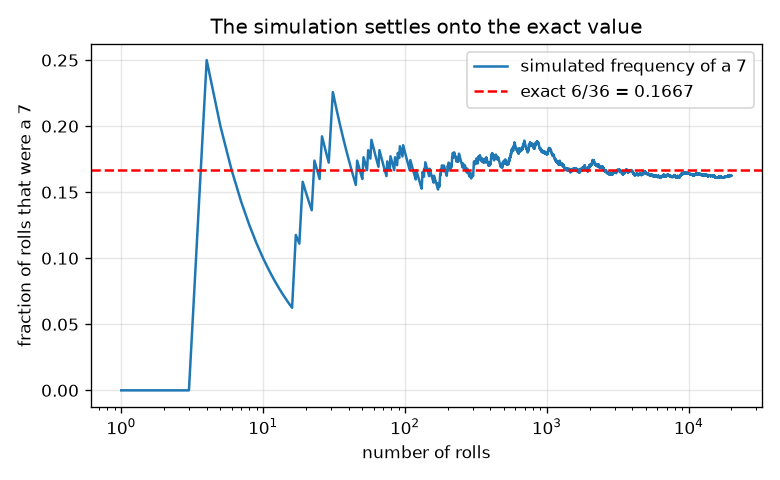
\includegraphics[width=0.85\linewidth]{figures/s01_convergence.png}\\\small The frequency of a 7 wobbles at first and settles onto the exact value 6/36.\end{center}

\subsection*{E. Worked example}
What is the probability that two fair dice add up to 7? Check it by counting all outcomes.
\begin{enumerate}[nosep]
\item List the outcomes: 6 x 6 = 36 equally likely pairs.
\item Favourable pairs: (1,6), (2,5), (3,4), (4,3), (5,2), (6,1). That is 6 pairs.
\item P(7) = 6 / 36 = 1/6 = 0.1667.
\item Sanity check: the 11 possible sums have 1,2,3,4,5,6,5,4,3,2,1 outcomes, which add up to 36, so the probabilities add up to 1.
\end{enumerate}
\textbf{Answer.} P(7) = 6/36 = 1/6, about 0.167: the most likely sum.

\subsection*{F. Questions}
\begin{enumerate}[nosep]
\item \textbf{Conceptual.} A friend says: 'Sums 6 and 8 each appear less often than 7, but 6 and 8 together appear more often than 7 and 12 together.' Is that right? Why is (1, 2) not the same outcome as (2, 1)?
\item \textbf{Numerical.} Find the probability that the sum of two dice is at least 10. Give your answer as a fraction and a decimal and check that it is between 0 and 1.
\item \textbf{Graph and simulation interpretation.} In the convergence figure, the frequency of a 7 after 10 rolls is far from 0.167 but after 20000 rolls it is very close. Does this mean the next roll is 'due' to be a 7 if the early frequency was too low?
\item \textbf{Design and optimisation challenge.} Design a game: you win if the sum is in a set S that you choose. Choose S so that the probability of winning is exactly 1/3, using as few different sums as you can, and say what trade-off you made.
\end{enumerate}

\section{Session 2: Counting rules: cards, birthdays and expected value}

\subsection*{A. Real-world problem}
Counting 36 outcomes is easy; counting 2.6 million poker hands is not. Do 23 people in a room really have a better than even chance of sharing a birthday? Could a school fair raffle ticket be priced so that the fair neither gains nor loses on average? All three questions are answered by the same idea: count cleverly, then divide. The raffle and prizes are made-up examples; this is education about chance, not betting advice.

\subsection*{B. Concept and theory}
Equally likely outcomes: P = favourable / total. If two events are independent, P(both) = P(first) x P(second); for example two sixes in a row has probability 1/6 x 1/6 = 1/36. A permutation is an ordered selection: there are n!/(n-k)! ways to pick and line up k of n objects. A combination ignores order: C(n, k) = n!/(k!(n-k)!), 'n choose k'. A 5-card hand is a combination, so there are C(52, 5) = 2,598,960 equally likely hands. Exactly one pair: choose the rank (13), its two suits C(4,2) = 6, three other different ranks C(12,3) = 220, and a suit for each, 4\textasciicircum{}3 = 64, giving 13 x 6 x 220 x 64 = 1,098,240 hands. A flush (five cards of one suit, straight flushes included): 4 x C(13,5) = 4 x 1287 = 5,148 hands. Birthday problem: P(all n birthdays differ) = (365/365)(364/365)...((365-n+1)/365), so P(shared) = 1 minus that. The expected value of a quantity that takes value v\_i with probability p\_i is the sum of v\_i p\_i, the long-run average. A game is fair when the expected net gain is 0.

\begin{itemize}[nosep]
\item n, k: number of objects, number chosen (count)
\item C(n, k): number of unordered selections (count)
\item P: probability (no unit (0 to 1))
\item N\_t: number of raffle tickets sold (tickets)
\item c: ticket price (Rs)
\item R: prize for the single winning ticket (Rs)
\item E: expected net gain per ticket (Rs)
\end{itemize}

\begin{equation*}
P(A\text{ and }B)=P(A)\,P(B)\quad(\text{independent events})
\end{equation*}

\begin{equation*}
{}^{n}P_{k}=\dfrac{n!}{(n-k)!},\qquad \binom{n}{k}=\dfrac{n!}{k!\,(n-k)!}
\end{equation*}

\begin{equation*}
P(\text{pair})=\dfrac{13\binom{4}{2}\binom{12}{3}4^{3}}{\binom{52}{5}},\qquad P(\text{flush})=\dfrac{4\binom{13}{5}}{\binom{52}{5}}
\end{equation*}

\begin{equation*}
P(\text{shared})=1-\prod_{i=0}^{n-1}\dfrac{365-i}{365}
\end{equation*}

\begin{equation*}
E=\sum_i v_i\,p_i,\qquad E_{\text{raffle}}=\dfrac{R}{N_t}-c\;\;\Rightarrow\;\; R_{\text{fair}}=N_t\,c
\end{equation*}

\begin{center}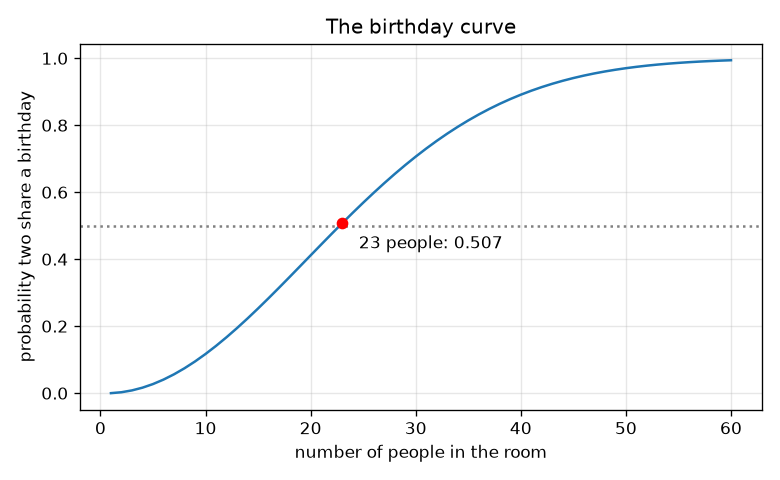
\includegraphics[width=0.85\linewidth]{figures/s02_birthday.png}\\\small The birthday curve crosses 0.5 at 23 people (0.507).\end{center}

\subsection*{E. Worked example}
A raffle sells 500 tickets at Rs 20. There is one prize. What prize makes the game fair for a buyer, and what is the expected net gain per ticket if the prize is Rs 5000?
\begin{enumerate}[nosep]
\item Each ticket wins with probability 1/500 and costs Rs 20.
\item Expected net gain E = R/500 - 20.
\item Fair means E = 0, so R = 500 x 20 = Rs 10000.
\item For R = 5000: E = 5000/500 - 20 = 10 - 20 = -Rs 10 per ticket.
\item Check: all 500 tickets bring in Rs 10000; paying out only Rs 5000 leaves Rs 5000 for the organiser, which is Rs 10 per ticket.
\end{enumerate}
\textbf{Answer.} The fair prize is Rs 10000; a Rs 5000 prize gives an expected net gain of -Rs 10 per ticket.

\subsection*{F. Questions}
\begin{enumerate}[nosep]
\item \textbf{Conceptual.} Why is a pair counted with C(4,2) = 6 and the three other cards with 4 x 4 x 4, rather than another combination? What would go wrong if you counted C(12,3) x C(4,1)?
\item \textbf{Numerical.} Find the probability of a flush (straight flushes included) in a 5-card hand and express it as '1 in about N'.
\item \textbf{Graph and simulation interpretation.} On the birthday curve, at about how many people does the curve first exceed 0.5, and is the curve straight? Why does it flatten near 1?
\item \textbf{Design and optimisation challenge.} Design a raffle: 1000 tickets at Rs 10 must raise Rs 3000 for charity, and a buyer's expected net gain must be -Rs 3 per ticket. What total prize money should you offer, and why can it not be one prize of Rs 10000?
\end{enumerate}

\section{Session 3: Monte Carlo simulation, its error, and when it fails}

\subsection*{A. Real-world problem}
When the exact count is too hard, we can play the game many times on a computer and see how often the event happens. But how close is that answer, how many plays do we need, and why can nobody simulate their way to a lottery jackpot with odds of 1 in 13,983,816? This session also checks whether a game you design is fair. It is education about chance, not betting advice.

\subsection*{B. Concept and theory}
Monte Carlo estimate: run N independent trials and set p\_hat = (trials where the event happened) / N. With a seeded generator the same seed repeats the same estimate. The estimate is random: for a true probability p its standard deviation (the standard error) is SE = sqrt(p(1-p)/N). About 95 percent of estimates lie within 1.96 SE of p. To get a 95 percent half-width e, we need N \textgreater{}= 1.96\textasciicircum{}2 p(1-p)/e\textasciicircum{}2; for p = 1/2 and e = 0.01 that is 9604 trials. Ten times better accuracy costs 100 times more trials. The law of large numbers says p\_hat settles near p, but separate trials have no memory: after 5 heads in a row the next flip is still 50:50 (the gambler's fallacy is believing otherwise). A lottery with 6 numbers out of 49 has C(49,6) = 13,983,816 equally likely draws, so one ticket wins the jackpot with probability 1/13,983,816. If a ticket costs c and the jackpot is J (smaller prizes ignored) the expected loss is c - J/13,983,816. For rare events the relative error is sqrt((1-p)/(pN)), so N must be about 1/(p x relative error squared): plain simulation needs hundreds of millions of draws just to find the jackpot probability to 30 percent. Exact counting, or importance sampling that samples the rare event on purpose and re-weights, is needed.

\begin{itemize}[nosep]
\item p: true probability of the event (no unit (0 to 1))
\item N: number of simulated trials (count)
\item p\_hat: simulated estimate of p (no unit (0 to 1))
\item SE: standard error of p\_hat (no unit)
\item e: wanted 95 percent half-width (no unit)
\item c, J: ticket price, jackpot (Rs)
\end{itemize}

\begin{equation*}
\hat p=\dfrac{\text{trials with the event}}{N}
\end{equation*}

\begin{equation*}
\mathrm{SE}=\sqrt{\dfrac{p(1-p)}{N}}
\end{equation*}

\begin{equation*}
N\ge\dfrac{1.96^{2}\,p(1-p)}{e^{2}}
\end{equation*}

\begin{equation*}
\binom{49}{6}=13\,983\,816,\qquad E_{\text{loss}}=c-\dfrac{J}{13\,983\,816}
\end{equation*}

\begin{equation*}
\dfrac{\mathrm{SE}}{p}=\sqrt{\dfrac{1-p}{pN}}\;\Rightarrow\;N\approx\dfrac{1}{p\,r^{2}}\ \text{for relative error } r
\end{equation*}

\begin{center}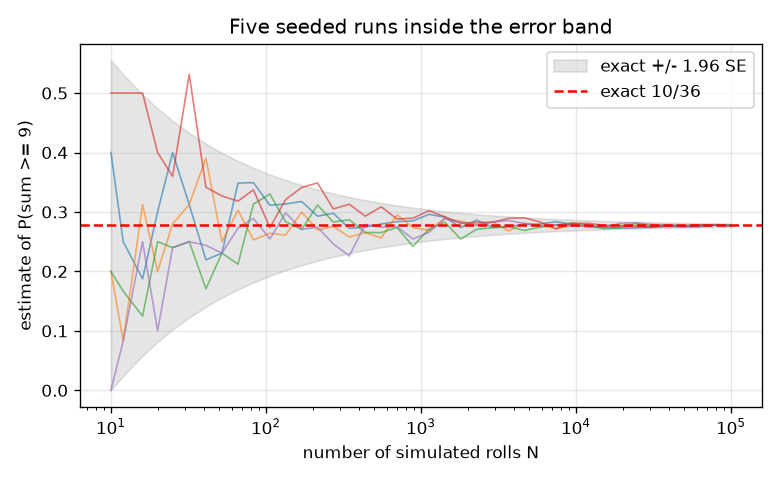
\includegraphics[width=0.85\linewidth]{figures/s03_error_band.png}\\\small Five seeded runs settle inside the 95 percent error band around 10/36.\end{center}

\subsection*{E. Worked example}
How many simulated trials are needed to estimate a probability near 0.5 to within plus or minus 0.01 (95 percent)? Then find the expected loss on a Rs 100 lottery ticket when the jackpot is Rs 10 crore (Rs 100,000,000), counting only the jackpot.
\begin{enumerate}[nosep]
\item Worst case p = 0.5: p(1-p) = 0.25.
\item N \textgreater{}= 1.96\textasciicircum{}2 x 0.25 / 0.01\textasciicircum{}2 = 3.8416 x 0.25 / 0.0001 = 9604 trials.
\item Check: SE = sqrt(0.25 / 9604) = 0.0051, and 1.96 x 0.0051 = 0.0100.
\item Lottery: P(jackpot) = 1 / 13,983,816. Expected jackpot winnings = 100,000,000 / 13,983,816 = Rs 7.15.
\item Expected loss = 100 - 7.15 = Rs 92.85 per ticket, ignoring smaller prizes.
\end{enumerate}
\textbf{Answer.} 9604 trials are enough for plus or minus 0.01 at p = 0.5; the Rs 100 ticket loses about Rs 92.85 per ticket on average (jackpot only).

\subsection*{F. Questions}
\begin{enumerate}[nosep]
\item \textbf{Conceptual.} A coin has landed heads 5 times in a row. A friend says tails is now due. Another says the coin must be biased. Who is right?
\item \textbf{Numerical.} You want to estimate P(two dice sum to at least 9) = 10/36 with a 95 percent half-width of 0.005. How many trials? How many if you want 0.0005?
\item \textbf{Graph and simulation interpretation.} In the band figure, a run leaves the grey band at N = 200 but is inside it at N = 20000. Is the simulation broken?
\item \textbf{Design and optimisation challenge.} Design a fair game: pay Rs 10, roll two dice, win a gross payout if the sum is at least 9. What payout makes it fair? Choose N to check it by simulation to within a standard error of 0.05 Rs and say what you would see for a payout of Rs 30.
\end{enumerate}

\section{Real-world mini-project}
\textbf{Design a fair game and check it by simulation.} Invent a dice game with a price and a payout. You pay a price, roll two dice, and win the gross payout when the sum is in a set you choose. Use exact counting to set the payout so that the expected net gain is 0, then use \texttt{simulate\_game} from Session 3 with a seed and a large N to check it. Also show that a payout 10 percent too small is caught by your simulation. This is education about chance, not a real gambling product.

\section{The path ahead}
\begin{enumerate}[nosep]
\item \textbf{Session 4: Importance sampling for a rare event.} An estimator of the probability that 8 dice all show 6 (exactly 6\textasciicircum{}-8) that samples biased dice and weights each sample.
\item \textbf{Session 5: The full poker table.} A function returning the count of every hand type for 5-card poker, checked against simulation.
\item \textbf{Session 6: Lottery prize tiers and honest expected value.} A table of the number of draws for each match count and the expected return for an illustrative prize list.
\item \textbf{Session 7: Conditional probability: Monty Hall.} A seeded simulation of the game with a confidence statement from the standard error.
\item \textbf{Session 8: Animate convergence like the Target.} An animation of simulated dice-sum frequencies and a birthday curve converging with 95 percent bands.
\end{enumerate}

\section{Answers and hints}

\subsection*{Session 1}
\begin{enumerate}[nosep]
\item \textbf{Conceptual.} Hint: Count the outcomes of each sum and add. Solution: Sums 6 and 8 have 5 + 5 = 10 outcomes; 7 and 12 together have 6 + 1 = 7 outcomes, so yes. (1, 2) and (2, 1) are different outcomes (first die 1 and second die 2, or the other way round); listing both is what makes all 36 outcomes equally likely and gives the sum 3 two ways, which is why 3 is twice as likely as 2.
\item \textbf{Numerical.} Hint: Count the outcomes for sums 10, 11 and 12 using c(s) = 6 - \textbar{}s - 7\textbar{}. Solution: c(10) = 3, c(11) = 2, c(12) = 1, so 6 favourable outcomes. P = 6/36 = 1/6 = 0.167. It is between 0 and 1, and it is the same as P(7), which makes sense because the counts 3 + 2 + 1 equal 6.
\item \textbf{Graph and simulation interpretation.} Hint: Think about what settles: the fraction or the counts? Solution: No. Each roll is independent and still has probability 1/6 of being a 7. The fraction settles because the early surplus or shortage is spread over more and more rolls, not because later rolls compensate. The size of the wobble falls roughly like one over the square root of n; Session 3 makes this exact.
\item \textbf{Design and optimisation challenge.} Hint: You need 12 favourable outcomes out of 36. Solution: You need 12 favourable outcomes out of 36. One choice is the sums 4, 7 and 10: 3 + 6 + 3 = 12, so S = \{4, 7, 10\} wins with probability 12/36 = 1/3. A single sum cannot do it because the largest count is 6, and two sums give at most 6 + 5 = 11. Trade-off: fewer sums means simpler rules but smaller reachable probabilities. Assumption: fair dice.
\end{enumerate}

\subsection*{Session 2}
\begin{enumerate}[nosep]
\item \textbf{Conceptual.} Hint: Each of the three other cards can independently be any of 4 suits, and the ranks must all be different. Solution: The two paired cards are an unordered choice of 2 suits from 4, so C(4,2) = 6. The three other cards have different ranks (C(12,3) ways) and each can have any of 4 suits independently, so 4\textasciicircum{}3 = 64. Using C(12,3) x C(4,1) would force all three cards to share one suit, so it would miss most hands.
\item \textbf{Numerical.} Hint: Use 4 x C(13, 5) over C(52, 5), with math.comb. Solution: C(13,5) = 1287, so 4 x 1287 = 5148 flush hands out of 2,598,960. P = 5148/2598960 = 0.001981, which is about 1 in 505. Sanity check: it is far smaller than the probability of a pair (0.4226), as expected for a hand that needs five cards of one suit.
\item \textbf{Graph and simulation interpretation.} Hint: Read where the dot crosses the dotted 0.5 line; think about what 1 - P(all different) does as P(all different) shrinks. Solution: It first exceeds 0.5 at 23 people (0.507; with 22 it is 0.476). The curve is not straight: it is S-shaped. The probability of all different birthdays is a product of numbers below 1, which shrinks faster and faster at first (more pairs appear with each new person) and then slowly, so P(shared) approaches 1 without reaching it before 366 people.
\item \textbf{Design and optimisation challenge.} Hint: Expected prize value per ticket = price + expected net gain. Solution: Expected prize value per ticket must be 10 - 3 = Rs 7, so total prize money is 1000 x 7 = Rs 7000 and the organiser keeps 10000 - 7000 = Rs 3000. One prize of Rs 10000 would make the expected net gain 10 - 10 = 0, a fair game, and raise nothing on average. Trade-off: one big prize is exciting but variable; many small prizes give a steadier experience for the same expected value.
\end{enumerate}

\subsection*{Session 3}
\begin{enumerate}[nosep]
\item \textbf{Conceptual.} Hint: Compare the chance of 5 heads from a fair coin with the information the next flip carries. Solution: For a fair coin the next flip is still 50:50, because flips are independent: the simulation after 5 heads gives 0.50 heads. The first friend commits the gambler's fallacy. The second is not certain either: 5 heads in a row has probability 1/32 = 0.031 for a fair coin, which happens often enough in a long sequence that it is weak evidence of bias. More flips would help.
\item \textbf{Numerical.} Hint: N = 1.96\textasciicircum{}2 p (1 - p) / e\textasciicircum{}2. Solution: p(1-p) = 0.2778 x 0.7222 = 0.2006. For e = 0.005: N = 3.8416 x 0.2006 / 0.000025, about 30,800 (30,828 with full precision). For e = 0.0005 (ten times smaller) N is 100 times larger: about 3,082,800. Sanity check: ten times the accuracy costs 100 times the trials.
\item \textbf{Graph and simulation interpretation.} Hint: What fraction of runs should leave a 95 percent band? Solution: No. A 95 percent band is left by about 5 percent of runs at any given N, so a run can step outside occasionally, especially at small N where the band is wide and the normal approximation is rough. What matters is that over many runs about 95 percent stay inside, and that the spread falls like 1/sqrt(N). The checkpoint tests this with 200 seeds.
\item \textbf{Design and optimisation challenge.} Hint: p = 10/36; fair payout = price / p. The standard deviation of one play is about Rs 16. Solution: Fair payout = 10 / (10/36) = Rs 36. For payout 30 the expected net gain is 10/36 x 30 - 10 = -Rs 1.67. One play has a standard deviation of about Rs 16, so N = (16/0.05)\textasciicircum{}2, about 100,000 trials or more; with N = 200000 the checkpoint finds a standard error near Rs 0.04 and a mean near -1.63. A fair game shows a mean within 3 standard errors of 0. Trade-off: more trials cost time. Assumption: fair dice.
\end{enumerate}

\section{How to join}
Read \texttt{CONTRIBUTING.md} in the repository, then pick an issue labelled \texttt{good first issue}. Repository: \url{https://github.com/KrunalPanchal1995/openodds}

\end{document}
